\chapter{Einleitung}
Quantenstrukturen, wie sie heutzutage hergestellt werden können, eröffnen neue Möglichkeiten im Bereich der ultraschnellen Elektronik und Photonik. Solche Strukturen lassen sich in aller Regel als \emph{offene} Systeme beschreiben. Es findet ein Austausch von lokal erhaltenen Fermionen -- die Erhaltung wird durch eine lokale Kontinuitätsgleichung beschrieben -- mit der Umgebung statt. Die Umgebung besteht dabei aus mindestens zwei verschiedenen Partikel-Reservoirs. In diesem Fall kann also ein Nicht-Gleichgewichtszustand erreicht werden, beispielsweise durch das Anlegen einer Spannung. Das zu untersuchende System besitzt eine endliche Ausdehnung im Raum. Es muss im Nicht-Gleichgewichtsfall folglich ein Strom durch die Oberfläche als Rand des Systems fließen. Wir beschränken uns hier auf eindimensionale Quantenstrukturen, für die also die interessante Physik in einer Dimension stattfindet. Dabei wollen wir den Strom der Teilchen, also den quantenmechanischen Transport beschreiben. Dies geschieht allgemein in verschiedenen Anwendungsfällen (Hydrodynamik, Aerodynamik, Elektronik, Neutronentransport, \dots) mit Hilfe einer die Dynamik beschreibenden Differentialgleichung. Hierfür werden Randbedingungen benötigt. Eben diese Randbedingungen definieren den offenen (oder auch geschlossenen) Charakter des Systems.

\chapter{Entwicklung}
\section{Herleitung der Liouville-von-Neumann Gleichung}

Die Liouville-von-Neumann Gleichung erhält man aus der Liouville-Gleichung wie folgt.
\begin{align}
  \partial_t \hat{\rho} &= \frac{i}{\hbar}\left[\hat{\rho} , H\right] \\
  \underbrace{\bra{x} \partial_t \hat{\rho} \ket{y}}_{\equiv \partial_t \rho(x,y)} &= \bra{x}\ket{\frac{i}{\hbar}\left[\hat{\rho} , H\right]y} \\
   &= \frac{i}{\hbar} \sum_k p_k ( \underbrace{\bra{x}\ket{\Psi_k}}_{\equiv \Psi_k(x)}\bra{\Psi_k}\ket{Hy} - \bra{x}\ket{H\Psi_k}\underbrace{\bra{\Psi_k}\ket{y}}_{\equiv \Psi_k^*(y)} )
\end{align}
Mit dem Hamiltonoperator für ein einzelnes Teilchen in einer Dimension in Ortsdarstellung
\begin{align}
  \left[ -\frac{\hbar^2}{2m}\frac{\partial^2}{\partial x^2} + V(x) \right] \Psi(x) = \bra{x}\ket{H\Psi} \equiv \mathcal{L}(x)\Psi(x)
\end{align}
folgt mit $H^{\dagger} = H$
\begin{align}
  \partial_t \rho(x,y) &= \frac{i}{\hbar} \sum_k p_k \left( \Psi_k(x)\mathcal{L}^*(y)\Psi_k^*(y) - \mathcal{L}(x)\Psi_k(x)\Psi_k^*(y) \right) \\
  &= \frac{i}{\hbar}  (\mathcal{L}^*(y) - \mathcal{L}(x)) \sum_k p_k \left( \Psi(x)\Psi^*(y) \right) \\
  &= \frac{i}{\hbar}  (\mathcal{L}^*(y) - \mathcal{L}(x)) \bra{x}\left(\sum_k p_k  \ket{\Psi_k}\bra{\Psi_k} \right)\ket{y} \\
  &= \frac{i}{\hbar}  (\mathcal{L}^*(y) - \mathcal{L}(x))\rho(x,y)
\end{align}
Wir definieren noch
\begin{align}
  \mathcal{L}(x,y) &\equiv \mathcal{L}(x) - \mathcal{L}^*(y)\\
   &= -\frac{\hbar^2}{2m}\left( \partial_x^2 - \partial_y^2 \right) + V(x) - V^*(y)
\end{align}
und erhalten die Liouville-von-Neumann Gleichung im Ortsraum
\begin{equation}
  \partial_t \rho(x,y) = \frac{1}{i\hbar} \mathcal{L}(x,y) \rho(x,y) \; .
\end{equation}
Es lassen sich zwei Fälle unterscheiden:
\begin{itemize}
  \item Der stationäre Fall mit $\partial_t \rho(x,y,t) = 0$
  \item der allgemeinere transiente Fall $\partial_t \rho(x,y,t) \neq 0$.
\end{itemize}

\section{Schwerpunkt- und Relativkoordinaten}
Wir führen die Schwerpunkt und Relativkoordinaten
\begin{align}
  &r \equiv \frac{x+y}{2} \qquad &q \equiv x-y \\
  \Leftrightarrow\qquad &x = r+\frac{q}{2} \qquad &y = r-\frac{q}{2}
\end{align}
ein. Die Ableitungen transformieren sich dabei gemäß
\begin{align}
  \partial_r \partial_q  &= \partial_r \left( \frac{\partial}{\partial x} \frac{\partial x}{\partial q} + \frac{\partial}{\partial y} \frac{\partial y}{\partial q}\right) \\
   &= \left( \frac{\partial}{\partial x} \frac{\partial x}{\partial r} + \frac{\partial}{\partial y} \frac{\partial y}{\partial r}\right) \left( \frac{\partial}{\partial x} \frac{1}{2} + \frac{\partial}{\partial y} \frac{-1}{2}\right)\\
    &= \left( \frac{\partial}{\partial x} 1 + \frac{\partial}{\partial y} 1\right) \left( \frac{\partial}{\partial x} \frac{1}{2} + \frac{\partial}{\partial y} \frac{-1}{2}\right)\\
   &= \frac{1}{2}\partial_x \partial_x - \frac{1}{2}\partial_x \partial_y + \frac{1}{2}\partial_y \partial_x - \frac{1}{2}\partial_y \partial_y \\
  &=  \frac{1}{2}(\partial_x^2 - \partial_y^2) \; ,
\end{align}
wobei im letzten Schritt der Satz von Schwarz genutzt wird. Damit ergibt sich der transformierte Liouville Operator zu
\begin{align}
  \mathcal{L}(r,q) = -\frac{\hbar^2}{m} \partial_r\partial_q + \underbrace{V\left(r+\frac{q}{2}\right) - V^*\left(r-\frac{q}{2}\right)}_{\equiv \tilde{B}(r,q)}
\end{align}
Mit der Umbenennung
\begin{align*}
  \rho \longrightarrow u \\
  r \longrightarrow \tilde{x} \\
  q \longrightarrow \tilde{y} \\
  t \longrightarrow \tilde{t}
\end{align*}
lautet die LvN Gleichung nun
\begin{align}
  i\hbar\partial_{\tilde{t}} u(\tilde{x},\tilde{y})+\frac{\hbar^2}{m}\operatorname{div}(A\nabla u(\tilde{x},\tilde{y})) -  \tilde{B}(\tilde{x},\tilde{y}) u(\tilde{x},\tilde{y}) = 0
\end{align}

\section{Charakteristische Einheiten}
Zunächst wird die  \lvn in eine einheitenlose Form gebracht.
\begin{align}
    i\frac{\hbar}{V_0}\partial_{\tilde{t}}\, u(\tilde{x},\tilde{y})+\frac{\hbar^2}{mV_0}\operatorname{div}(A\nabla u(\tilde{x},\tilde{y})) - \frac{\tilde{B}(\tilde{x},\tilde{y})}{V_0} u(\tilde{x},\tilde{y}) = 0
\end{align}
Energien werden in Einheiten von $V_0$ gemessen, welche wir im weiteren Verlauf als die Potentialbarriere $V_0 = \SI{0.1768}{\electronvolt}$ wählen werden.

Wir führen folgende Skalierung ein, um nun auch Zeiten und Orte einheitenlos zu behandeln.
\begin{align}
  \left(\begin{array}{c}\tilde{x}\\\tilde{y}\end{array}\right) &= \xi \left(\begin{array}{c}x\\y\end{array}\right)   & \xi &= \sqrt{\frac{\hbar^2}{mV_0}} \\
  \tilde{t} &= \tau t   & \tau &= \frac{\hbar}{V_0}
\end{align}
Damit folgt
\begin{align}
  \partial_{\tilde{t}} &= \frac{\partial}{\partial (\tau t)} = \tau^{-1} \partial_t = \frac{V_0}{\hbar} \partial_t \\
  \partial_{\tilde{x}}^2 &= \frac{\partial^2}{(\partial (\xi x))^2} = \xi^{-2} \partial_x^2 = \frac{mV_0}{\hbar^2} \partial_x² \; ,
\end{align}
sodass die \lvn die Form
\begin{align}
  i \partial_t u(x,y)+\operatorname{div}(A\nabla u(x,y)) - B(x,y) u(x,y) = 0
\end{align}
annimmt. Hierbei ist
\begin{align}
  B(x,y) \equiv \frac{\tilde{B}(x,y)}{V_0} = \frac{V\left(x+\frac{y}{2}\right) - V^*\left(x-\frac{y}{2}\right)}{V_0}
\end{align}
eingeführt worden. Die Skalierung lässt sich berechnen, indem die effektive Masse als konstant
\begin{align}
  m = 0.063 m_0 =  0.063\cdot\SI{9.1e-31}{\kilogram}
\end{align}
angenommen wird. Damit ergibt sich folgende Skalierung zwischen SI-Einheiten und den hier eingeführten einheitenlosen Größen.
\begin{align}
  V_0 &= \SI{0.1768}{\electronvolt} \\
  \xi &= \SI{6.57e-10}{\meter}
 \\
  \tau &= \SI{3.72e-15}{\second}

\end{align}

\section{Randbedingungen}


\section{Potential}
Das Verfahren soll am Beispiel einer resonanten Tunneldiode (RTD) getestet werden. Dessen durch die Materialkomposition GaAs/AlGaAs resultierender Potentialverlauf ist in Abbildung \ref{fig:pot1} gezeigt.
\begin{figure}
  \centering
  \includegraphics[width=0.7\textwidth]{plots/potential.pdf}
  \caption{Potentialverlauf der RTD.}
  \label{fig:pot1}
\end{figure}
Die eingezeichneten Längen wählen wir wie in (paper) zu
\begin{align}
  L_1 &= \SI{6}{\nano\meter}\\
  L_2 &= \SI{5}{\nano\meter}\\
  L_U &= \SI{30}{\nano\meter} \; .
\end{align}
Hierin ist $L_U$ die Länge, über der die Spannung $U$ abfällt. Auch hier lassen sich wieder zwei Fälle unterscheiden.
\begin{itemize}
  \item Der Gleichgewichtsfall $U=0$. Hier kann als Randbedingung auf beiden Seiten die Fermi-Dirac-Statistik \ref{eq:fd_statistic} angenommen werden.
  \item Der Nicht-Gleichgewichtsfall $U>0$. Hier sind lediglich die \emph{inflow}-Bedingungen für positive Geschwindigkeiten am linken- und negative Geschwindigkeiten am rechten Rand des Rechengebietes bekannt.
\end{itemize}

\section{Strom- und Ladungsträgerdichte}
Aus der Dichtematrix $\rho(r,q,t)$ lassen sich Strom- und Ladungsträgerdichte ableiten. Es gilt
\begin{align}
  j(r,t) &= \frac{\hbar}{m}\Im{\partial_q \rho(r,q,t)|_{q=0}} \\
  n(r,t) &= \Re{\rho(r,q,t)|_{q=0}} \; .
\end{align}


\section{Wigner Funktion}
Es ist mit $\bra{x}\ket{\Psi} = \Psi(x)$
\begin{equation}
  P(x,p) \equiv \frac{1}{\pi\hbar} \int_{-\infty}^{\infty} \bra{x+y}\hat{\rho} \ket{x-y} \E{2ipy/\hbar} \diff y
\end{equation}
die Wigner-Funktion gleich der Wigner-transformierten des Dichteoperators $\hat{\rho}$. Die Wigner Transformation ist eine invertierbare Abbildung
\begin{align}
  W\; :\; L(\HR,\HR)  \rightarrow & \text{Phasenraum}^* \\
   \hat{G} \mapsto & g(x,p) = \int_{-\infty}^{\infty} \bra{x-s/2}\hat{G} \ket{x+s/2} \E{ips/\hbar} \diff s
\end{align}
